%%%%%%%%%%%%%%%%%%%%%%%%%%%%%%%%%%%%%%%%%%%%%%%%%%%%%%%%%%%%%%%%%%%%%%%%%%%%%%%%%%%%%%%%%%%%%%%%%%%
%%%%%%%%%%%%%%%%%%%%%%%%%%%%%%%%%%%%%%%%%%%%%%%%%%%%%%%%%%%%%%%%%%%%%%%%%%%%%%%%%%%%%%%%%%%%%%%%%%%
\chapter{Introducci\'on}

La poblaci\'on mundial est\'a envejeciendo aceleradamente, lo que se debe en gran parte a la 
mejor\'ia en la atenci\'on de la salud durante el \'ultimo siglo, traducida en vidas m\'as 
largas y saludables. Sin embargo, este logro tambi\'en ha tenido como resultado un aumento en el 
n\'umero de personas con enfermedades no transmisibles, incluida la demencia.
Por otro lado, todav\'ia son incipientes las investigaciones para identificar 
factores de riesgo modificables de la demencia.
\cite{PlanAlzheimer04}




La demencia es un síndrome de naturaleza cr\'onica y progresiva, caracterizado 
por el deterioro de las funciones cognoscitivas y de la conducta, lo que ocasiona 
discapacidad y dependencia.
\cite{PlanAlzheimer04}

%%%%%%%%%%%%%%%%%%%%%%%%%%%%%%%%%%%%%%%%%%%%%%%%%%%%%%%%%%%%%%%%%%%%%%%%%%%%%%%%%%%%%%%%%%%%%%%%%%%

El objetivo de este trabajo es explorar la hip\'otesis de estacionariedad en registros
de PSG en adultos mayores con Deterioro Cognitivo y de
un grupo control.

A tyrav\'es de una metodolog\'ia de estudio de casos, se describen posibles diferencias entre 
registros 
de PSG en sujetos de ambos grupos, lo que sugieren su utilizaci\'on como
como marcadores de uso cl\'inico en el diagn\'ostico del DC en adultos mayores.

%
%El estudio y diagnóstico de una gran cantidad de enfermedades depende de nuestra habilidad para
%registrar y analizar se\~nales electrofisiol\'ogicas. 
%
%Se suele asumir que estas se\~nales son complejas: no lineales, no estacionarias y sin equilibrio 
%por naturaleza. Pero usualmente no se comprueban formalmente estas propiedades.
%
%Correlaci\'on inter-hemisf\'erica durante el sueño MOR del Adulto Mayor con Deterioro Cognitivo.

%\begin{figure}[h]
%\centering
%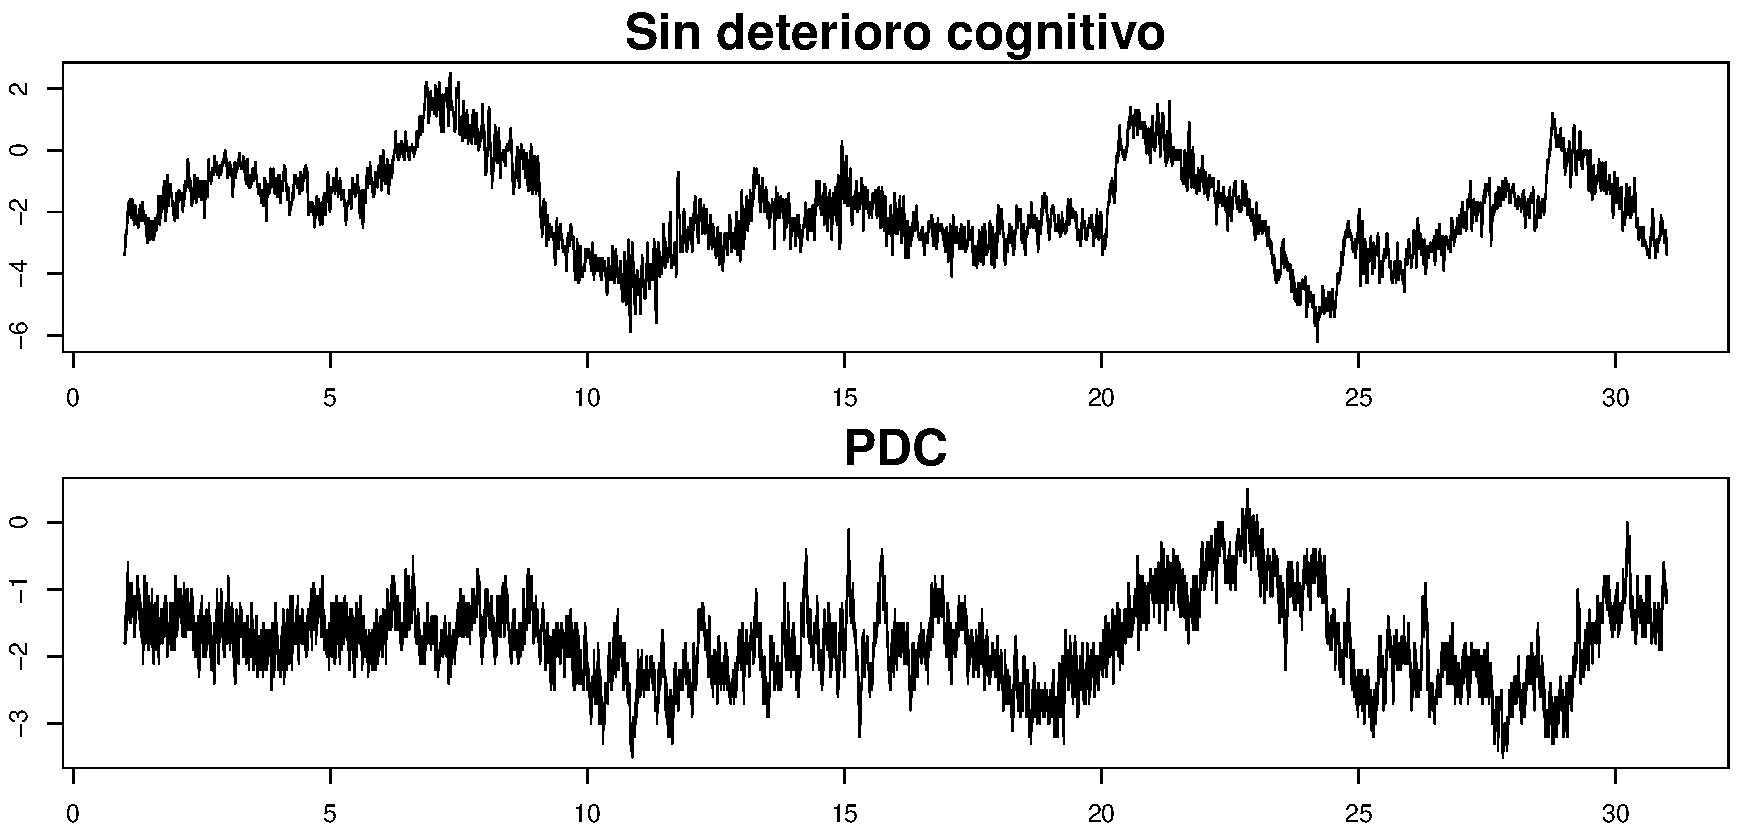
\includegraphics[width=.8\linewidth]{graficaintro.pdf}
%\caption{Adaptado de V\'azquez-Tagle y colaboradores (2016)}
%\end{figure}

%%%%%%%%%%%%%%%%%%%%%%%%%%%%%%%%%%%%%%%%%%%%%%%%%%%%%%%%%%%%%%%%%%%%%%%%%%%%%%%%%%%%%%%%%%%%%%%%%%%
%%%%%%%%%%%%%%%%%%%%%%%%%%%%%%%%%%%%%%%%%%%%%%%%%%%%%%%%%%%%%%%%%%%%%%%%%%%%%%%%%%%%%%%%%%%%%%%%%%%